%%%%%%%%%%%%%%%%%%%%%%%%%%%%%%%%%%%%%%%%%
% fphw Assignment
% LaTeX Template
% Version 1.0 (27/04/2019)
%
% This template originates from:
% https://www.LaTeXTemplates.com
%
% Authors:
% Class by Felipe Portales-Oliva (f.portales.oliva@gmail.com) with template 
% content and modifications by Vel (vel@LaTeXTemplates.com)
%
% Template (this file) License:
% CC BY-NC-SA 3.0 (http://creativecommons.org/licenses/by-nc-sa/3.0/)
%
%%%%%%%%%%%%%%%%%%%%%%%%%%%%%%%%%%%%%%%%%

%----------------------------------------------------------------------------------------
%	PACKAGES AND OTHER DOCUMENT CONFIGURATIONS
%----------------------------------------------------------------------------------------

\documentclass[
	12pt, % Default font size, values between 10pt-12pt are allowed
	%letterpaper, % Uncomment for US letter paper size
	%spanish, % Uncomment for Spanish
]{fphw}

% Template-specific packages
\usepackage[utf8]{inputenc} % Required for inputting international characters
\usepackage[T1]{fontenc} % Output font encoding for international characters
\usepackage{mathpazo} % Use the Palatino font
\usepackage{setspace}

\usepackage{graphicx} % Required for including images

\usepackage{booktabs} % Required for better horizontal rules in tables

\usepackage{listings} % Required for insertion of code

\usepackage{enumerate} % To modify the enumerate environment
\usepackage{caption}
\usepackage{parskip}% http://ctan.org/pkg/parskip
%----------------------------------------------------------------------------------------
%	ASSIGNMENT INFORMATION
%----------------------------------------------------------------------------------------

\title{AULA 1 - Introdução} % Assignment title

\author{AVC, JPP, PC} % Student name

\date{} % Due date

\institute{Pontifícia Universidade Católica do Rio de Janeiro \\ Departamento de Informática} % Institute or school name

\class{Programação Modular (INF1301)} % Course or class name

\professor{Flavio Bevilacqua} % Professor or teacher in charge of the assignment

%----------------------------------------------------------------------------------------

\begin{document}

\maketitle % Output the assignment title, created automatically using the information in the custom commands above

%----------------------------------------------------------------------------------------
%	ASSIGNMENT CONTENT
%----------------------------------------------------------------------------------------
\begin{doublespace}
    As vantagens do modelo modular incluem: particionar problemas (subdividí-los, divide and conquer) e permitir que diversos indivíduos contribuam para a solução de um mesmo problema. Tudo que é computável pode ser desenvolvido.
    
    \noindent Módulo genérico -> void*
    
    \noindent Vantagens da modularidade:

    \begin{itemize}

        \item Permite vencer barreiras de complexidade.

        \item Facilita o trabalho em grupo atravéz da paralelização de tarefas.

        \item Permite reuso do código.

        \item Permite a criação de acervos de módulos que fazem parte de determinados assuntos.

        \item Facilita a administração de baselines com módulos já testados.

        \item Facilita o desenvolvimento incremental: agrega, testa, agrega testa, agrega, testa, etc.

        \item Facilita  aprimoramento individual, no sentido de que um aspecto pode ser modificado sem que o resto do projeto seja afetado ou tenha que ser modificado.

        \item Reduz o tempo de compilação. Isso porque somente os módulos que foram modificados devem ser recompilados.

    \end{itemize}

    Teste unitário é o teste individual de cada módulo feito pelo desenvolvedor. Teste de integração é o teste do executável, o conjunto dos módulos.

    Baseline é o estado testado e estável do executável, depois que todos os testes unitários eo teste de integração obtiveram sucesso.

    Se algo é atualizado/modificado novos testes devem ser executados. Ao final dos testes, se tudo estiver correto, uma nova baseline é estabelecida.

    \textbf{Princícpios da Modulardiade}

    \begin{enumerate}

        \item Módulo

              Definição física: unidade independente de compilação.

              Definição lógica: um único conceito.

        \item Elementos de uma aplicação

              Hierarquia: Sistemas -> Programas -> Módulos -> Classes (smente se for orientado a objeto) -> Funções -> Blocos de código -> Linha de comando

              Artefato é qualquer elemento versionado criado ao longo de um processo de desenvolvimento. Por exemplo: programa, documento, ata, relatório.

              Construto (build) é uma versão, mesmo que incompleta, da aplicação. Algo que é funcional e apresentável. Todo construto é um artefato, mas nem todo artefato é um construto.

        \item Interface

              Definição: mecanismo de troca de dados, estados e comandos entre elementos de uma aplicação.

              OBS: a interface somente ocorre no mesmo nível da hierarquia dos elementos deuma aplicação. Portanto, interfaces ocorrem entre sistemas, entre programas, entre módulos entre funções, etc.

              Formas de interface: Sistemas se comunicam por APIs e arquivos. Módulos se comunicam por funções de acesso. Blocos de código se comunicam por variáveis globais.

              Relacionamento Cliente-Servidor

              \begin{figure}[h]
                  \centering
                  
\includegraphics[width=0.75\textwidth]{clienteservidor.png}
                  \caption*{M2 pode ser cliente do servidor M1.}
              \end{figure}

              Caso especial: callback

              \begin{figure}[h!]
                  \centering
                  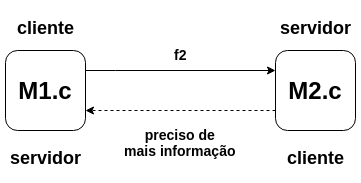
\includegraphics[width=0.55\textwidth]{callback1.png}
                  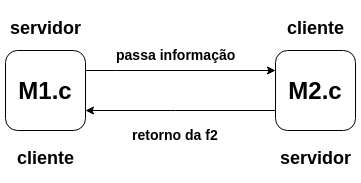
\includegraphics[width=0.55\textwidth]{callback2.png}
              \end{figure}

              \pagebreak

              Interface fornecida por terceiros:

              \begin{figure}[h]
                  \centering
                  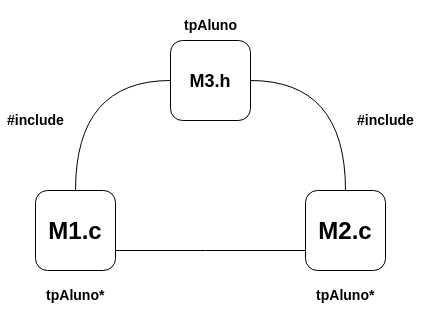
\includegraphics[width=0.62\textwidth]{interfacefornecida.png}
                  \caption*{Caso em que dois módulos usam a mesma struct. Em vez de duplicar o código, devemos criar um módulo de definição (.h) e dar include deste módulo em ambos os módulos de implementação (.c).}
              \end{figure}

    \end{enumerate}
\end{doublespace}


% \section*{Question 1}

% \begin{problem}
% What is the airspeed velocity of an unladen swallow?
% \end{problem}
% \begin{center}
%     \includegraphics[width=0.5\columnwidth]{swallow.jpg} % Example image
% \end{center}

% %------------------------------------------------

% \subsection*{Answer}

% While this question leaves out the crucial element of the geographic origin of the swallow, according to Jonathan Corum, an unladen European swallow maintains a cruising airspeed velocity of \textbf{11 metres per second}, or \textbf{24 miles an hour}. The velocity of the corresponding African swallows requires further research as kinematic data is severely lacking for these species.

% %----------------------------------------------------------------------------------------

% \section*{Question 2}

% \begin{problem}
% How much wood would a woodchuck chuck if a woodchuck could chuck wood?

% \medskip

% \begin{enumerate}[(\itshape a\normalfont)] % Sub-questions styled as italic letters
%     \item Suppose ``chuck" implies throwing.
%     \item Suppose ``chuck" implies vomiting.
% \end{enumerate}
% \end{problem}

% %------------------------------------------------

% \subsection*{Answer}

% \begin{enumerate}[(\itshape a\normalfont)] % Sub-questions styled as italic letters
%     \item According to the Associated Press (1988), a New York Fish and Wildlife technician named Richard Thomas calculated the volume of dirt in a typical 25--30 foot (7.6--9.1 m) long woodchuck burrow and had determined that if the woodchuck had moved an equivalent volume of wood, it could move ``about \textbf{700 pounds (320 kg)} on a good day, with the wind at his back".

%     \item A woodchuck can ingest 361.92 cm\textsuperscript{3} (22.09 cu in) of wood per day. Assuming immediate expulsion on ingestion with a 5\% retainment rate, a woodchuck could chuck \textbf{343.82 cm\textsuperscript{3}} of wood per day.
% \end{enumerate}

% %----------------------------------------------------------------------------------------

% \section*{Question 3}

% \begin{problem}
% Identify the author of Equation \ref{eq:bayes} below and briefly describe it in Latin.

% \medskip

% \begin{equation}\label{eq:bayes}
%     P(A|B) = \frac{P(B|A)P(A)}{P(B)}
% \end{equation}

% \smallskip
% \end{problem}

% %------------------------------------------------

% \subsection*{Answer}

% Lorem ipsum dolor sit amet, consectetur adipiscing elit. Praesent porttitor arcu luctus, imperdiet urna iaculis, mattis eros. Pellentesque iaculis odio vel nisl ullamcorper, nec faucibus ipsum molestie. Sed dictum nisl non aliquet porttitor. Etiam vulputate arcu dignissim, finibus sem et, viverra nisl. Aenean luctus congue massa, ut laoreet metus ornare in. Nunc fermentum nisi imperdiet lectus tincidunt vestibulum at ac elit. Nulla mattis nisl eu malesuada suscipit.

% %----------------------------------------------------------------------------------------

% \section*{Question 4 (bonus marks)}

% \begin{problem}
% The table below shows the nutritional consistencies of two sausage types. Explain their relative differences given what you know about daily adult nutritional recommendations.

% \bigskip

% \begin{center}
%     \begin{tabular}{l l l}
%         \toprule
%         \textit{Per 50g} & Pork  & Soy   \\
%         \midrule
%         Energy           & 760kJ & 538kJ \\
%         Protein          & 7.0g  & 9.3g  \\
%         Carbohydrate     & 0.0g  & 4.9g  \\
%         Fat              & 16.8g & 9.1g  \\
%         Sodium           & 0.4g  & 0.4g  \\
%         Fibre            & 0.0g  & 1.4g  \\
%         \bottomrule
%     \end{tabular}
% \end{center}

% \medskip
% \end{problem}

% %------------------------------------------------

% \subsection*{Answer}

% Lorem ipsum dolor sit amet, consectetur adipiscing elit. Praesent porttitor arcu luctus, imperdiet urna iaculis, mattis eros. Pellentesque iaculis odio vel nisl ullamcorper, nec faucibus ipsum molestie. Sed dictum nisl non aliquet porttitor. Etiam vulputate arcu dignissim, finibus sem et, viverra nisl. Aenean luctus congue massa, ut laoreet metus ornare in. Nunc fermentum nisi imperdiet lectus tincidunt vestibulum at ac elit. Nulla mattis nisl eu malesuada suscipit.

% %----------------------------------------------------------------------------------------

% \section*{Question 5 (bonus marks)}

% \begin{problem}
% \lstinputlisting[
%     caption=Luftballons Perl Script, % Caption above the listing
%     label=lst:luftballons, % Label for referencing this listing
%     language=Perl, % Use Perl functions/syntax highlighting
%     frame=single, % Frame around the code listing
%     showstringspaces=false, % Don't put marks in string spaces
%     numbers=left, % Line numbers on left
%     numberstyle=\tiny, % Line numbers styling
% ]{luftballons.pl}

% \begin{enumerate}
%     \item How many luftballons will be output by the Listing \ref{lst:luftballons} above?
%     \item Identify the regular expression in Listing \ref{lst:luftballons} and explain how it relates to the anti-war sentiments found in the rest of the script.
% \end{enumerate}

% \end{problem}

% %------------------------------------------------

% \subsection*{Answer}

% \begin{enumerate}
%     \item 99 luftballons.
%     \item Lorem ipsum dolor sit amet, consectetur adipiscing elit. Praesent porttitor arcu luctus, imperdiet urna iaculis, mattis eros. Pellentesque iaculis odio vel nisl ullamcorper, nec faucibus ipsum molestie. Sed dictum nisl non aliquet porttitor. Etiam vulputate arcu dignissim, finibus sem et, viverra nisl. Aenean luctus congue massa, ut laoreet metus ornare in. Nunc fermentum nisi imperdiet lectus tincidunt vestibulum at ac elit. Nulla mattis nisl eu malesuada suscipit.
% \end{enumerate}

% %----------------------------------------------------------------------------------------

\end{document}
